\chapter{基于递推最小二乘的积分滑模控制方法研究}
\section{引言}
从第二章分析中可以知道,精密直线运动平台本质上也是一种非线性系统,尤其是其摩擦力、定位力、模型参数摄动、纹波扰动以及外部不确定扰动等均呈现出一定的非线性特性,因此,采用非线性的反馈控制器提高精密直线运动平台系统的整体控制性能显得很有必要,尤其是在超精密运动控制领域,抑制上述扰动带来的影响是提高运动控制性能的关键环节。近年来,滑模控制由于其控制律中含有具有开关特性的鲁棒项(符号函数及其变种),在处理PMLSMs诸多扰动因素时表现出优势\cite{wang2015modified,slotine1983tracking,burton1986continuous,tseng2010chattering,zhang2013design,lee2017adaptive}。但是,符号函数在原点附近的不连续会造成抖振,甚至可能造成系统不稳定或激发更多的不期望的模态,严重影响精密直线运动平台系统位置跟踪精度\cite{tseng2010chattering}。另一方面,由于缺乏对系统扰动的精确建模,传统的滑模控制方法在高速、高精度运动控制系统中不能完全满足要求,往往需要与额外的扰动补偿方法相结合。在精密直线运动平台控制系统中,前馈控制常常与反馈控制相结合,前者主要用来提高系统跟踪精度和补偿系统扰动,后者常用来维持系统稳定并一定程度上抑制系统的扰动,提高系统稳态精度。对于精密运动控制领域经常采用的三阶轨迹来说,前馈控制器主要在加减速段发挥作用,而反馈控制器主要在匀速段发挥作用。经典的前馈控制方法主要是基于系统的逆模型,但是往往需要提前辨识系统的模型,而且对模型辨识的精度要求极高,对于复杂的系统往往很难做到精确辨识,因此自适应的逆模型前馈控制显得很有必要。

本章首先介绍了滑模控制和递推最小二乘(Recursive Least Square, RLS)算法的基本原理,然后用积分滑模控制(Integral Sliding Mode Control, ISMC)作为反馈部分,用RLS实现逆模型的自适应前馈控制。为了能够补偿定位力带来的扰动,进一步对基于RLS的自适应逆模型前馈方法进行了改进,提出了一种基于改进型RLS的积分滑模控制方法,该方法将定位力的主要频率部分引入到RLS的回归向量中,从而进一步提高系统位置跟踪精度。
\section{滑模控制基本原理}
考虑单输入动态系统\cite{slotine2006应用非线性控制}
\begin{equation}
\label{4单输入动态系统}
x^{(n)}=f(\textbf{\textit{x}})+b(\textbf{\textit{x}})u
\end{equation}
式中,标量$x$是控制系统输出(如精密直线运动平台的位置),标量$u$是控制信号输入(比如电机的出力),向量$\textbf{\textit{x}}=[x,\dot{x},\dots,x^{n-1}]^T$为状态向量。$f(\textbf{\textit{x}})$通常表示一个非线性函数,用来表示系统的扰动,虽然不能精确知道,但一般都认为它的上界是$\textbf{\textit{x}}$的连续函数。$b(\textbf{\textit{x}})$也认为不能精确已知,但是其不确定性也认为是有界的,比如PMLSMs模型参数摄动等。

为了使有限控制$u$实现较为理想的跟踪任务,系统的期望状态的初始值$\textbf{\textit{x}}_d(0)$必须满足
\begin{equation}
\label{初态}
\textbf{\textit{x}}_d(0)=\textbf{\textit{x}}(0)
\end{equation}
即当$t=0$时控制系统输出与目标轨迹一致,这一条件在实际精密运动控制中基本都会满足,因为系统的位置和速度不会突变。

记跟踪误差为$e=x_d-x$,则跟踪误差向量为 $\textbf{\textit{e}}=\textbf{\textit{x}}_d-\textbf{\textit{x}}=[e \quad\dot {e} \quad\cdots \quad e^{n-1}]^T$。用标量方程$s(\textbf{\textit{e}};t)=0$定义n维状态空间中的滑模曲面$S(t)$
\begin{equation}
\label{滑模面0}
s(\textbf{\textit{e}},t)=\left(\frac{\text{d}}{\text{dt}}+\lambda\right)^{n-1}\textbf{\textit{e}}
\end{equation}
式中,$\lambda$为一正常数。$n$表示系统的阶数,比如机械系统,大部分会是二阶系统,即$n=2$,此时
\begin{equation}
\label{滑模面1}
s=\lambda e+\dot{e}
\end{equation}
即$s$仅是状态轨迹,即系统跟踪位置误差和速度误差的线性加权;$\lambda$为一正常数。


给定初始状态(\ref{初态}),跟踪问题$\textbf{\textit{x}}\equiv\textbf{\textit{x}}_d$则等价于当$t$\textgreater$0$时,通过一定的控制手段使系统状态轨迹能够始终停留在曲面$S(t)$上。实际上$s\equiv0$本质上为一种线性微分方程的表示,假定系统状态轨迹的初态满足式(\ref{初态}),则其唯一解为$\tilde{\textbf{\textit{x}}}\equiv0$。因此,通过一定的控制方式实现跟踪$n$维向量$\textbf{\textit{x}}_d$的问题可巧妙地转化为如何使标量$s$恒为零的问题。

更进一步,通过选择式(\ref{4单输入动态系统})中的控制信号$u$,使得状态轨线在曲面$S(t)$之外满足下式
\begin{equation}
\label{收敛条件}
\frac{1}{2}\frac{\text{d}}{\text{dt}}s^2\leq-\eta\left|s\right|
\end{equation}
从而保证$s$恒为零的问题简化为一阶问题,其中$\eta$为一正常数。如图\ref*{滑动条件}所示,系统状态轨线只要能够满足式(\ref{收敛条件}),系统状态轨线就会不断趋向于曲线$S(t)$,曲面$S(t)$就可以认为是一个不变集。系统状态轨线沿曲面$S(t)$运动的状态我们称为滑动模态。
%满足式(\ref{收敛条件})的曲面$S(t)$称为滑动曲面,当系统状态轨迹进入滑动曲面后,我们可以说系统进入了滑动模态,或滑动模。
\begin{figure}[H]
	\centering
	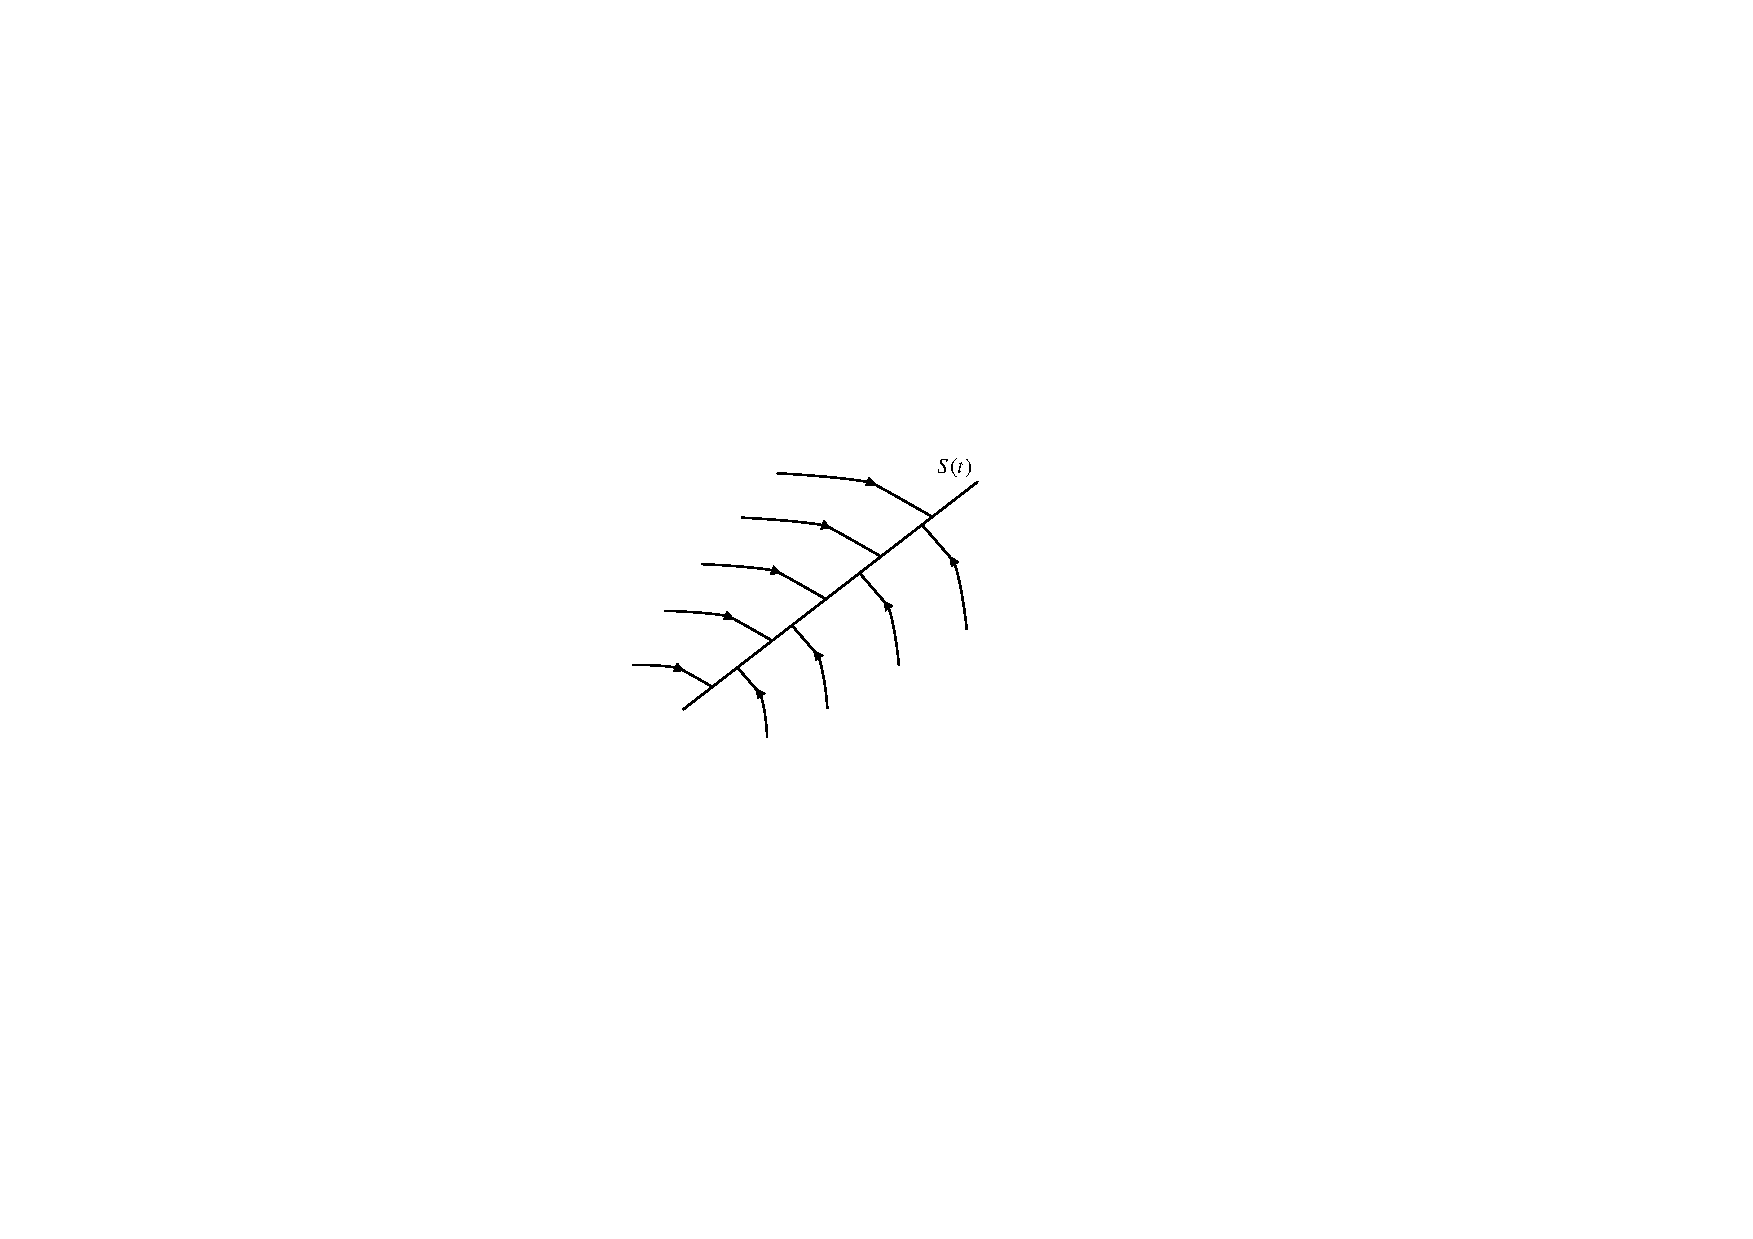
\includegraphics[width=10cm]{figures/滑动条件.pdf}
	\caption{滑动条件}
	\label{滑动条件}
\end{figure}
\begin{comment}
实际上,即使式(\ref*{初态})不满足,即初始时刻,系统输出与系统目标轨迹不一致,也就是说,系统不满足零状态,系统轨线仍然能够在小于$s(t=0)/\eta$的有限时间内到达曲面$S(t)$。总的来说,这种通过设计滑模面$S(t)$,并合理设计控制律$u$以使系统状态轨迹收敛到滑模面上的方法,成为滑模控制,是一种有效的容易实现的鲁棒控制方法。
\end{comment}
\section{递推最小二乘原理}
在介绍递推最小二乘原理之前,有必要先介绍最小二乘法。最小二乘法主要解决的问题是,对于像式(\ref{最小二乘})一样的表示,
\begin{equation}
\label{最小二乘}
y=\left[\begin{matrix}
x_{1} & \cdots & x_{n}
\end{matrix}\right]\left[\begin{matrix}
\theta_{1} \\
\vdots \\
\theta_{n}
\end{matrix}\right]
\end{equation}
其中$x$和$y$为一系列观测得到的数据,通过观测得到的$x$和$y$,求解其对应的估计参数$\symbf{\Theta}$的过程。可以用矩阵表示如下
\begin{equation}
\left[\begin{matrix}
y_{1} \\
\vdots \\
y_{k}
\end{matrix}\right]=\left[\begin{matrix}
\symbf{\phi}_{1}^{T} \\
\vdots \\
\symbf{\phi}_{k}^{T}
\end{matrix}\right] \symbf{\Theta}
\end{equation}
式中,
$k$表示观测到的数据个数;
$\symbf{\phi}_{i}^{T}=\left[\begin{matrix}x_{1}^{i} & \cdots & x_{n}^{i}\end{matrix}\right] \in \mathbb{R}^{1 \times n}$,表示第$i$组观测数据的输入量;

$y_i$表示第$i$组观测数据的输出量;

$\symbf{\Theta}=\left[\begin{matrix}\theta_{1} \\ \vdots \\ \theta_{n}\end{matrix}\right] \in \mathbb{R}^{n \times 1}$,为待估计参数。

记$\symbf{\Phi}_{k}=\left[\begin{matrix}\symbf{\phi}_{1}^{T} \\ \vdots \\ \symbf{\phi}_{k}^{T}\end{matrix}\right] \in \mathbb{R}^{k \times n}, \symbf{Y}_{k}=\left[\begin{matrix}y_{1} \\ \vdots \\ y_{k}\end{matrix}\right] \in \mathbb{R}^{k \times 1}$,则有
\begin{equation}
\label{3.8}
\symbf{\Phi}_{k}^{T}\left(\symbf{Y}_{k}-\symbf{\Phi}_{k} \hat{\symbf{\Theta}}_{k}\right)=0
\end{equation}
则通过方程(\ref{3.8}),即可求得最小二乘参数$\symbf{\Theta}_k$的估计,
\begin{equation}
\label{3.9}
\hat{\symbf{\Theta}}_{k}=\left(\symbf{\Phi}_{k}^{T} \symbf{\Phi}_{k}\right)^{-1} \symbf{\Phi}_{k}^{T} \symbf{Y}_{k}
\end{equation}
通过上述过程,可以发现,如果我们能够得到$x$和$y$的观测值,我们可以通过最小二乘方法求出$y$和$x$之间的函数关系。但是最小二乘法要求计算之前就能够得到所有的观测值,也就是说所有的数据都要提前准备好,这要求较大的存储空间,也影响计算速度,不利于实时在线的计算和补偿。因此,递推最小二乘应运而生。

递推最小二乘原理的根本目的是希望能够得到一种估计值的递推形式,比如$\hat{\symbf{\Theta}}_k=\hat{\symbf{\Theta}}_{k-1}+\Delta\hat{\symbf{\Theta}}_k$。下面是详细的推导过程:

最小二乘法的一般解如式(\ref{3.9})所示,这里分别表示$\symbf{\Phi}_{k}^{T} \symbf{\Phi}_{k}$和$\symbf{\Phi}_{k}^{T} \symbf{Y}_{k}$,令$\symbf{P}_{k}^{-1}=\symbf{\Phi}_{k}^{T} \symbf{\Phi}_{k}$,则有
\begin{equation}
\label{公式1}
\begin{aligned}
\symbf{\Phi}_{k}^{T} \symbf{\Phi}_{k}&=\left[\begin{matrix}
\symbf{\phi}_{1} & \cdots & \symbf{\phi}_{k}
\end{matrix}\right]\left[\begin{matrix}
\symbf{\phi}_{1}^{T} \\
\vdots \\
\symbf{\phi}_{k}^{T}
\end{matrix}\right]\\
&=\sum_{i=1}^{k} \symbf{\phi}_{i} \symbf{\phi}_{i}^{T}\\
&=\sum_{i=1}^{k-1} \symbf{\phi}_{i} \symbf{\phi}_{i}^{T}+\symbf{\phi}_{k} \symbf{\phi}_{k}^{T}\\
&=\symbf{P}_{k-1}^{-1}+\symbf{\phi}_{k} \symbf{\phi}_{k}^{T}
\end{aligned}
\end{equation}
同时,
\begin{equation}
\label{公式2}
\begin{aligned}
\symbf{\Phi}_{k}^{T} \symbf{Y}_{k}&=\left[\begin{matrix}
\symbf{\phi}_{1} & \cdots & \symbf{\phi}_{k}
\end{matrix}\right]\left[\begin{matrix}
y_{1} \\
\vdots \\
y_{k}
\end{matrix}\right]\\
&=\sum_{i=1}^{k} \symbf{\phi}_{i} y_{i}\\
&=\sum_{i=1}^{k-1} \symbf{\phi}_{i} y_{i}+\symbf{\phi}_{k} y_{k}\\
&=\symbf{\Phi}_{k-1}^{T} \symbf{Y}_{k-1}+\symbf{\phi}_{k} y_{k}
\end{aligned}
\end{equation}

此外,根据最小二乘法的一般解可以得到
\begin{equation}
\label{公式3}
\begin{matrix}
\hat{\symbf{\Theta}}_{k-1}=\left(\symbf{\Phi}_{k-1}^{T} \symbf{\Phi}_{k-1}\right)^{-1} \symbf{\Phi}_{k-1}^{T} \symbf{Y}_{k-1} \\
\Rightarrow \hat{\symbf{\Theta}}_{k-1}=\symbf{P}_{k-1} \symbf{\Phi}_{k-1}^{T} \symbf{Y}_{k-1} \\
\Rightarrow \symbf{P}_{k-1}^{-1} \hat{\symbf{\Theta}}_{k-1}=\symbf{\Phi}_{k-1}^{T} \symbf{Y}_{k-1}
\end{matrix}
\end{equation}

结合公式(\ref{公式1})$\sim$公式(\ref{公式3}),再次回顾最小二乘法的一般解,可以得出下面的推导
\begin{equation}
\begin{aligned}
\hat{\symbf{\Theta}}_{k}&=\left(\symbf{\Phi}_{k}^{T} \symbf{\Phi}_{k}\right)^{-1} \symbf{\Phi}_{k}^{T} \symbf{Y}_{k}\\
%&=\symbf{P}_{K} \symbf{\Phi}_{k}^{T} \symbf{Y}_{k}\\
&=\symbf{P}_{k}\left(\symbf{\Phi}_{k-1}^{T} \symbf{Y}_{k-1}+\symbf{\phi}_{k} \symbf{y}_{k}\right) \\
&=\symbf{P}_{k}\left(\symbf{P}_{k-1}^{-1} \hat{\symbf{\Theta}}_{k-1}+\symbf{\phi}_{k} \symbf{y}_{k}\right) \\
&=\symbf{P}_{k}\left[\left(\symbf{P}_{k}^{-1}-\symbf{\phi}_{k} \symbf{\phi}_{k}^{T}\right) \hat{\symbf{\Theta}}_{k-1}+\symbf{\phi}_{k} \symbf{y}_{k}\right] \\
%&=\hat{\symbf{\Theta}}_{k-1}-\symbf{P}_{k} \symbf{\phi}_{k} \symbf{\phi}_{k}^{T} \hat{\symbf{\Theta}}_{k-1}+\symbf{P}_{k} \symbf{\phi}_{k} \symbf{y}_{k}\\
&=\hat{\symbf{\Theta}}_{k-1}+\symbf{P}_{k} \symbf{\phi}_{k}\left(y_{k}-\symbf{\phi}_{k}^{T}\hat{\symbf{\Theta}}_{k-1}\right)\\
&=\hat{\symbf{\Theta}}_{k-1}+\symbf{K}_{k} \varepsilon_{k}\\
\end{aligned}
\end{equation}
至此,估计参数写成了$\hat{\symbf{\Theta}}_{k}=\hat{\symbf{\Theta}}_{k-1}+\Delta\symbf{\Theta}$的形式,其中$\Delta\symbf{\Theta}=\symbf{K}_k\varepsilon_{k}$。

综合上述的推导过程,这里可以进一步地给出递推最小二乘法的原理公式:
\begin{equation}
\label{RLS}
\left\{
\begin{aligned}
\hat{\symbf{\Theta}}_{k}&=\hat{\symbf{\Theta}}_{k-1}+\symbf{K}_{k} \varepsilon_{k}\\
\symbf{K}_{k}&=\symbf{P}_{k} \symbf{\phi}_{k}\\
\varepsilon_{k}&={y_{k}}-{\symbf{\phi}_{k}^{T} \hat{\symbf{\Theta}}_{k-1}}\\
\symbf{P}_{k}&=\left(\symbf{P}_{k-1}^{-1}+\symbf{\phi}_{k} \symbf{\phi}_{k}^{T}\right)^{-1}
\end{aligned}
\right.
\end{equation}
这里需要说明的是,$y_k$为标量、$\symbf{\phi}_{k}^{T}$、$\symbf{\Theta}_k$、$\symbf{\Theta}_{k-1}$都为向量。值得注意的是,公式(\ref{RLS})还无法通过编程实现递推最小二乘算法进行参数$\symbf{\Theta}$的估计。还要对其中的$\symbf{P}_k$进行进一步地求解。这里首先给出一个矩阵引逆定理(证明略):
假设矩阵$\symbf{A}\in \mathbb{C}^{N\times N}$,$\symbf{C}\in\mathbb{C}^{N\times N}$,均为非奇异矩阵,矩阵$\symbf{B}\in\mathbb{C}^{N\times M}$,$\symbf{D}\in\mathbb{C}^{M\times N}$,则矩阵$\symbf{A}+\symbf{BCD}$具有逆矩阵:
\begin{equation}
\label{引逆定理}
[\symbf{A}+\symbf{B C D}]^{-1}=\symbf{A}^{-1}-\symbf{A}^{-1} \symbf{B}\left[\symbf{C}^{-1}+\symbf{D} \symbf{A}^{-1} \symbf{B}\right]^{-1} \symbf{D} \symbf{A}^{-1}
\end{equation}
根据矩阵引逆定理(\ref{引逆定理}),
设 $\symbf{A}=\symbf{P}_{K-1}^{-1}, \symbf{B}=\symbf{\phi}_{k}, \symbf{C}=1, \symbf{D}=\symbf{\phi}_{k}^{T}$
则有
\begin{equation}
\label{逆}
\begin{aligned}
\symbf{P}_{k}&=\left(\symbf{P}_{k-1}^{-1}+\symbf{\phi}_{k} \symbf{\phi}_{k}^{T}\right)^{-1}\\
&=[\symbf{A}+\symbf{B C D}]^{-1}\\
&=\symbf{A}^{-1}-\symbf{A}^{-1} \symbf{B}\left[\symbf{C}^{-1}+\symbf{D} \symbf{A}^{-1} \symbf{B}\right]^{-1} \symbf{D} \symbf{A}^{-1}\\
&=\symbf{P}_{k-1}-\symbf{P}_{k-1} \symbf{\phi}_{k}\left[1+\symbf{\phi}_{k}^{T} \symbf{P}_{k-1} \symbf{\phi}_{k}\right]^{-1} \symbf{\phi}_{k}^{T} \symbf{P}_{k-1}\\
&=\symbf{P}_{k-1}-\frac{\symbf{P}_{k-1} \symbf{\phi}_{k} \symbf{\phi}_{k}^{T} \symbf{P}_{k-1}}{1+\symbf{\phi}_{k}^{T} \symbf{P}_{k-1} \symbf{\phi}_{k}}
\end{aligned}
\end{equation}

将式(\ref{逆})带入式(\ref{RLS}),可以得到最终的递推最小二乘算法:
\begin{equation}
\label{RLS1}
\left\{
\begin{aligned}
\hat{\symbf{\Theta}}_{k}&=\hat{\symbf{\Theta}}_{k-1}+\symbf{K}_{k} \varepsilon_{k}\\
\symbf{K}_{k}&=\symbf{P}_{k} \symbf{\phi}_{k}\\
\varepsilon_{k}&={y_{k}}-{\symbf{\phi}_{k}^{T}\hat{\symbf{\Theta}}_{k-1}}\\
\symbf{P}_{k}&=\symbf{P}_{k-1}-\frac{\symbf{P}_{k-1} \symbf{\phi}_{k} \symbf{\phi}_{k}^{T} \symbf{P}_{k-1}}{1+\symbf{\phi}_{k}^{T} \symbf{P}_{k-1} \symbf{\phi}_{k}}
\end{aligned}
\right.
\end{equation}
其中,

$y_k$为输出观测值;

$\symbf{\phi}_k$为输入观测向量,也称回归向量;

$\hat{\symbf{\Theta}}_{k}$为待估计参数向量;

$\symbf{P}_k$为更新律。
至此,所得到的递推最小二乘算法可以直接通过编程实现。


\section{基于传统递推最小二乘的前馈控制器设计}
在光刻机工件台与掩模台运动控制系统中,由于高分辨率和高产率的需求,常常希望精密直线运动平台加速段的精度更高、整定时间更短,这时,往往只靠反馈控制器不能很好地实现这一目的,因此,将前馈补偿与反馈控制相结合成为了一种较为流行的控制架构。经典的前馈补偿方式为系统逆模型前馈,通过事先辨识好系统的模型参数,然后通过逆模型前馈的方式计算得到需要的力。但是这种方式,需要对模型参数事先进行辨识,而且要求的辨识精度较高,往往需要付出额外的人力物力成本。一种较好的策略是通过在线自适应的方式调整系统的逆模型前馈参数\cite{butler2012adaptive},这样对于提前辨识的参数精度要求不高,只需要一个粗略的初始值即可实现逆模型自适应前馈控制,本节重点研究基于递推最小二乘方法进行逆模型自适应前馈的策略,并将之与积分滑模控制相结合,实现精密直线运动平台的高性能控制。

传统递推最小二乘积分滑模系统控制框图如图\ref{传统RLS}所示,主要包含自适应逆模型前馈与积分滑模反馈两部分,下面具体介绍基于传统递推最小二乘的前馈控制器的设计。
% TODO: \usepackage{graphicx} required
\\
\begin{figure}[H]
	\centering
	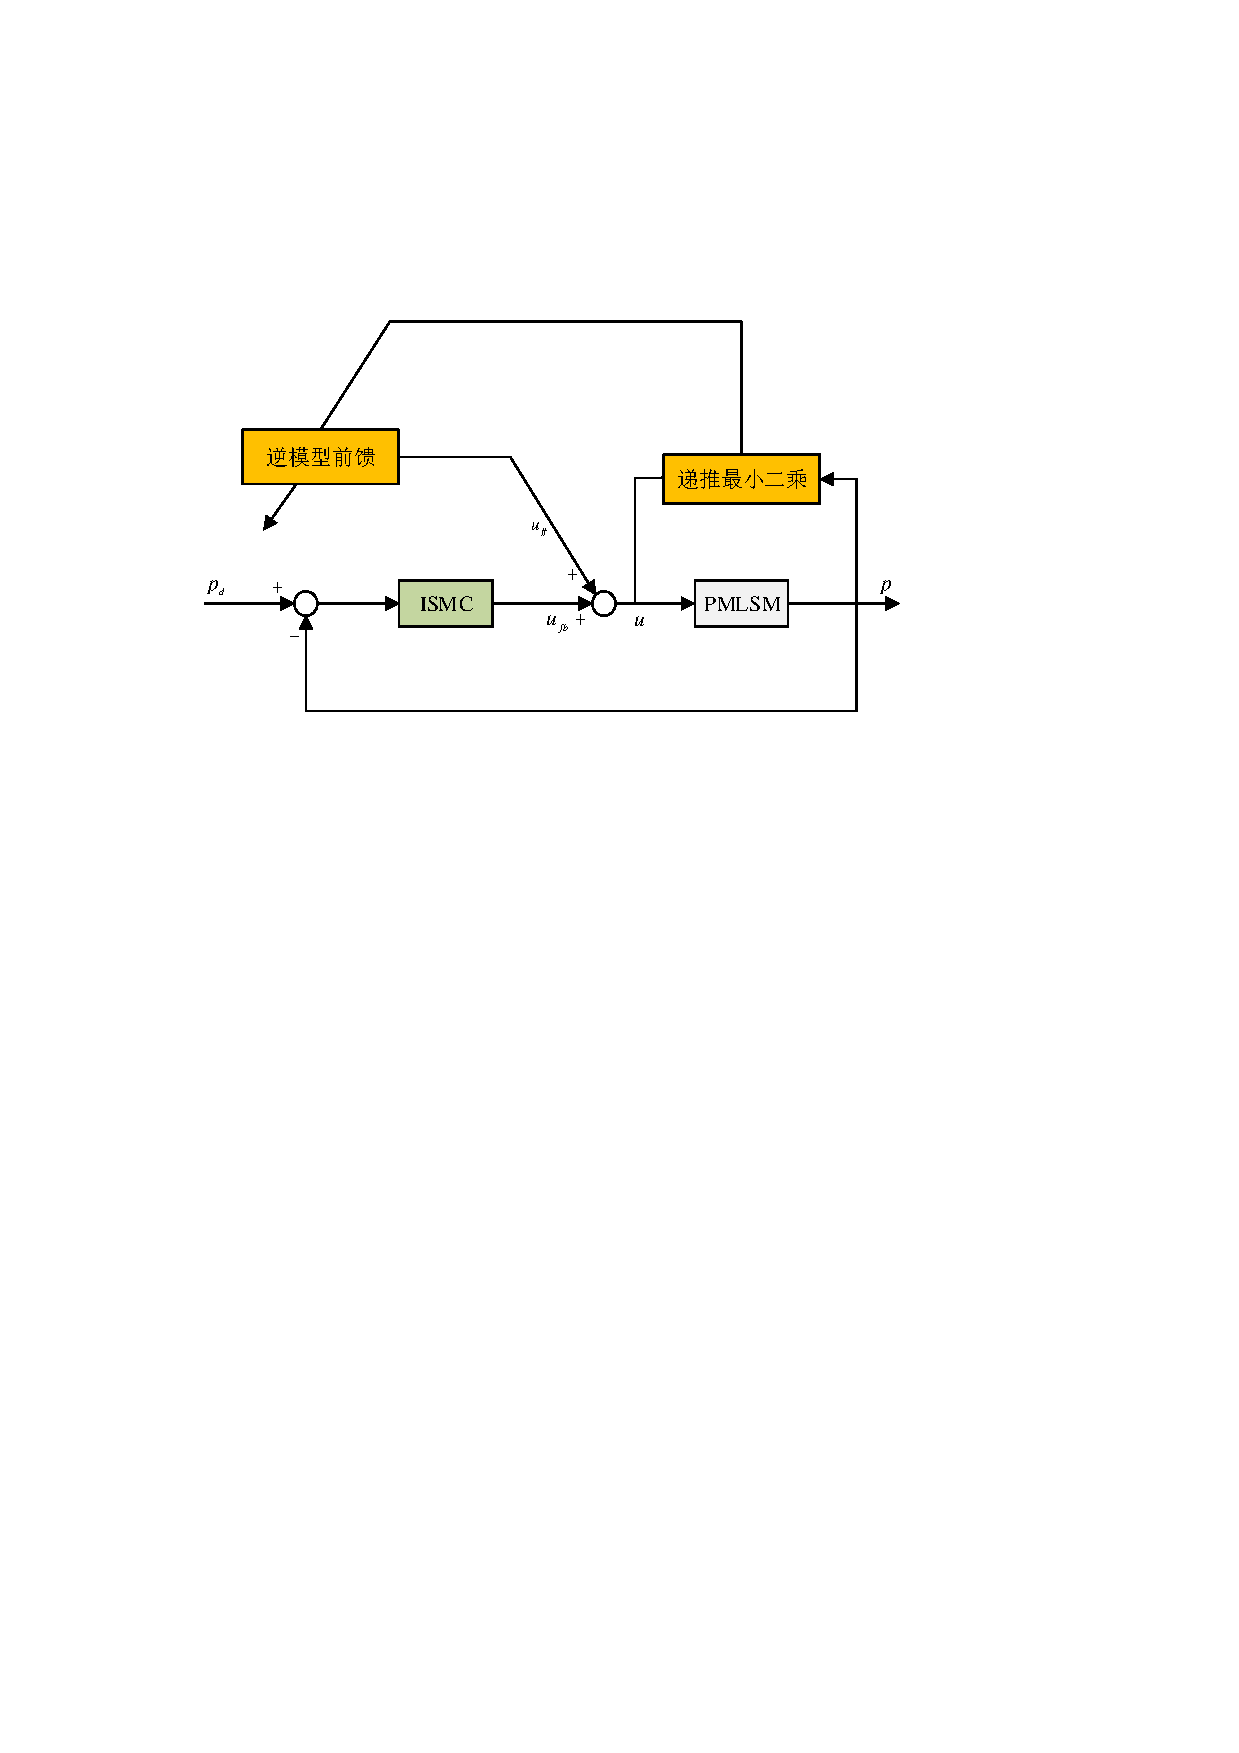
\includegraphics[width=12cm]{figures/RLSISMC2.pdf}
	\caption{传统递推最小二乘的积分滑模控制系统框图}
	\label{传统RLS}
\end{figure}

%\subsection{基于传统递推最小二乘的前馈控制器设计}

以经典的集中质量模型$1/(M_es^2+D_es+K_e)$为例,逆模型前馈控制信号可以表示为
\begin{equation}
\label{传统逆模型前馈}
u_{ff}=(M_es^2+D_es+K_e)p_d
\end{equation}
式中,$p_d$为系统位置参考轨迹。$M_e$、$D_e$和$K_e$为系统逆模型待确定的参数,$s$为拉普拉斯算子,表示微分。

如果将逆模型待确定的参数表示为向量的形式$\symbf{\Theta}=[M_e\,\, D_e\,\, K_e]^{T}$,则根据式(\ref{RLS1}),$\symbf{\Theta}$可以被估计为
\begin{equation}
\label{3.20}
\hat{\symbf{\Theta}}_{k}=\hat{\symbf{\Theta}}_{k-1}+\symbf{P}_{k} \symbf{\phi}_{k}\varepsilon_{k}
\end{equation}
式中,

$\hat{\symbf{\Theta}}_{k}$表示待确定参数向量的估计值;

$\symbf{P}_k$为自适应更新律,为一矩阵,可以表示为$\symbf{P}_{k}=\symbf{P}_{k-1}-\frac{\symbf{P}_{k-1} \symbf{\phi}_{k} \symbf{\phi}_{k}^{T} \symbf{P}_{k-1}}{1+\symbf{\phi}_{k}^{T} \symbf{P}_{k-1}\symbf{\phi}_{k}}$;

$\symbf{\phi}_{k}$为递推最小二乘的回归向量,即基向量,可以表示为$\symbf{\phi}_{k}=\left[\frac{d^{2} p_d}{d t^{2}} \,\,\frac{d p_d}{d t} \,\,p_d \right]^{T}$,这里指系统的三阶参考轨迹;

$\varepsilon_{k}$表示估计误差。

一旦$\symbf{\Theta}_k$的估计值$\hat{\symbf{\Theta}_k}$得到,就可以通过计算得出前馈控制器的估计输出指令
\begin{equation}
\label{3.21}
\hat{u_{ff}}=\hat{\symbf{\Theta}_k}^{T}\symbf{\phi}_{k}
\end{equation}
理想前馈控制器输出指令与估计得到的输出指令之间的差值可以表示为
\begin{equation}
\label{3.22}
\varepsilon_{k}^{'}=u_{ff}-\hat{u_{ff}}=\left[\symbf{\Theta}_k-\hat{\symbf{\Theta}_k}\right]^{T}\symbf{\phi}_{k}
\end{equation}
结合式(\ref{3.20})和式(\ref{3.22})以及文献\cite{landau1980extension}中定理2.1所表示的系统,$\varepsilon_{k}^{'}$又可假设为
\begin{equation}
\label{3.23}
\varepsilon_{k}^{'}=u_{ff}-\hat{u_{ff}}=Q\left[\Theta_k-\hat{\Theta_{k}}\right]^{T}\phi_{k}
\end{equation}
式中,$Q$为一离散的有理分式,根据波波夫超稳定性理论\cite{landau1980extension},如果$Q^{'}=Q-\frac{\lambda}{2}\,(0<\lambda<1)$严格正定,那么不管参数向量的估计初值$\hat{\symbf{\Theta}_0}$和自适应更新律初值$\symbf{P}_0$为何值,都有$\varepsilon_{k}^{'}$有界且
\begin{equation}
\label{3.24}
\lim _{k \rightarrow \infty} \varepsilon_{k}^{'}=0
\end{equation}

根据式(\ref{3.22})和式(\ref{3.23}),不难发现,在这里离散的有理传递函数$Q=1$,而且$Q^{'}=Q-\frac{\lambda}{2}>\frac{1}{2}$严格正定,因此,基于式(\ref{3.25})的递推最小二乘估计算法能够保证估计参数的收敛性。从图\ref{RLSISMC}
中可以看到,自适应前馈部分并未包含在系统的反馈回路中,因此,只要能够保证自身参数的收敛性,基于递推最小二乘估计的自适应前馈部分并不影响整个系统的闭环稳定性,闭环稳定性完全由积分滑模控制部分决定。
\begin{comment}
\subsection{基于积分滑模的反馈控制器设计}

精密直线运动平台的系统模型如式(\ref{2.14})所示,
$$
\begin{aligned}
\ddot{p}&=({{A}_{n}}+\Delta A)u_{fb}+L \\
&={A}_{n}u_{fb}+H  
\end{aligned}
$$
这里假设总扰动$H$有界,即$H\le\mu$,$\mu$为一正常数。$u_{fb}$表示反馈控制指令。

定义系统位置跟踪误差为
\begin{equation}
\label{3.25}
e=p_d-p
\end{equation}
可以得到误差对时间的导数为
\begin{equation}
\label{3.26}
\dot{e}=\dot{p_d}-\dot{p}
\end{equation}
滑模控制部分的设计主要包括两部分:滑模面的设计和控制律的设计。
这里设计滑模面为含积分项的滑模面
\begin{equation}
\label{3.27}
s=\lambda e+\beta\int_{}^{}e\text{d}t+\dot{e}
\end{equation}
式中,$\lambda$和$\beta$均为正常数。

根据式(\ref{3.26})和(\ref{3.27}),可以得出滑模面对时间的一阶导数为
\begin{equation}
\label{3.28}
\begin{aligned}
\dot{s}&=\lambda \dot{e}+\beta e+\ddot{e} \\ 
&=\lambda\dot{e}+\beta e+{{{\ddot{p}}}_{d}}-\ddot{p} \\ 
&=\lambda \dot{e}+\beta e+{{{\ddot{p}}}_{d}}-{{A}_{n}}u_{fb}-H  
\end{aligned}
\end{equation}
这里考虑到系统状态轨线的初始状态可能与目标轨迹的初始状态不一致,即系统可能不是零状态,因此需要一定的到达阶段才能保证系统状态轨线收敛到滑模面,为了方便,选定到达阶段的趋近律为等速趋近律
\begin{equation}
\label{3.29}
\dot{s}=-\eta\text{sgn}(s)
\end{equation}
式中,

$\text{sgn}(\cdot)$为符号函数;

$\eta$为正常数,满足$\eta\ge\mu$,主要决定到达阶段的趋近速率以及滑模控制的鲁棒性。

另一方面,设计滑模控制律为
\begin{equation}
\label{3.30}
u_{fb}=\frac{1}{A_n}\left(\lambda \dot{e}+\beta e+\ddot{p_d}+\eta\text{sgn}(s)\right)
\end{equation}
将式(\ref{3.30})代入式(\ref{3.28}),可得
\begin{equation}
\label{3.31}
\dot{s}=-\eta \text{sgn}(s)-H
\end{equation}

如前面提到的,基于递推最小二乘的积分滑模控制系统的闭环稳定性取决于积分滑模控制部分,这里为了证明其稳定性,根据Lyapunov稳定性理论,选择Lyapunov函数
\begin{equation}
\label{3.32}
V=\frac{1}{2}s^2
\end{equation}
两边对时间求导,即可得
\begin{equation}
\label{3.33}
\dot{V}=s\dot{s}
\end{equation}
将式(3.31)代入(3.33)中可以得到
\begin{equation}
\label{3.34}
\begin{aligned}
\dot{V}&=-\eta s\text{sgn}(s)-sH\\
&=-\eta\left|s\right|-sH\\
&\leq-\eta\left|s\right|+\mu\left|s\right|\\
&\leq-(\eta-\mu)\left|s\right|\\
&\leq 0
\end{aligned}
\end{equation}
取$\dot{V}\equiv0$,则$s\equiv0$,由LaSalle不变集定理可知,当$t\to\infty,s\to0$。至此,积分滑模反馈控制部分的渐近稳定性得以证明,反馈控制部分也设计完毕。
\end{comment}

\section{基于改进型递推最小二乘的积分滑模控制器设计}
\begin{comment}
在精密直线运动平台中,采用传统的基于递推最小二乘的积分滑模控制方法能够提高系统的位置跟踪精度,尤其是基于递推最小二乘的自适应逆模型前馈,能够有效地提高加速段的跟踪精度,同时减小系统从加速段进入匀速段的整定时间。但是正如第二章讨论的一样,由于精密直线运动平台本身的诸多非线性因素的影响,要进一步地提高系统的位置跟踪精度和扰动抑制能力,仅依赖逆模型前馈的积分滑模控制还有改进的空间。
\end{comment}




本节重点针对精密直线运动平台的定位力带来的扰动,在自适应前馈阶段引入了定位力的最大空间周期对应的扰动,对原有递推最小二乘的回归向量进行了改进,改进后的回归向量为$\symbf{\phi}_{k}^{'}=\left[\frac{d^{2} p}{d t^{2}} \,\,\frac{d p}{d t} \,\,p \,\,\text{sin}\left(2\pi p/\tau_m\right)\,\,\text{cos}\left(2\pi p/\tau_m\right)\right]^{T}$,其中,$\tau_m=2\tau/3=40/3\,\text{mm}$。改进之后的递推最小二乘可以分为两个部分:一是逆模型前馈部分,主要用来提高系统的瞬态响应速度;另一个是定位力补偿部分,用来补偿位置依赖的扰动对位置跟踪精度的影响。两部分都通过改进的递推最小二乘估计方法进行自适应调节,改进递推最小二乘积分滑模控制系统框图如图\ref{RLSISMC}所示。下面详细地介绍各部分的设计过程。
\begin{figure}[H]
	\centering
	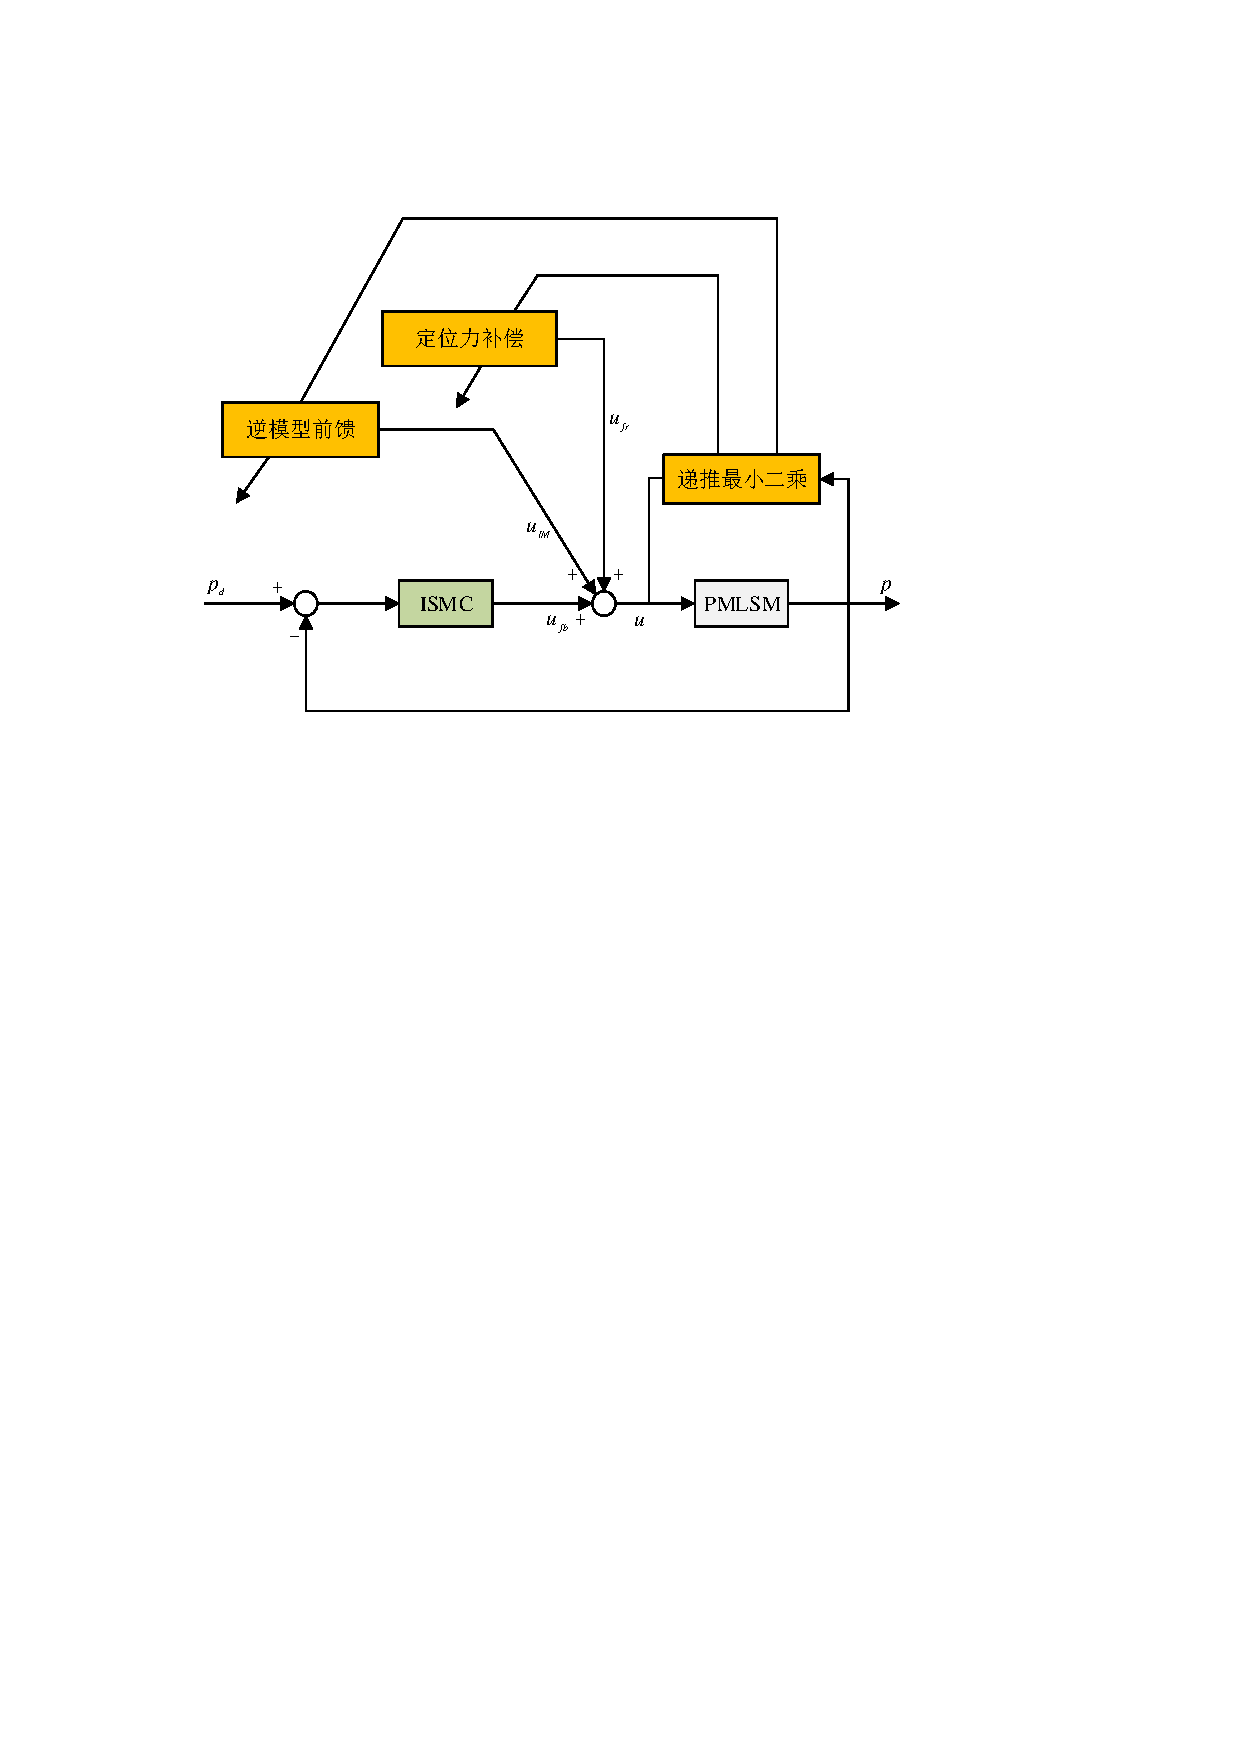
\includegraphics[width=12cm]{figures/RLSISMC系统框图.pdf}
	\caption{改进递推最小二乘积分滑模控制系统框图}
	\label{RLSISMC}
\end{figure}

\subsection{基于改进型递推最小二乘的前馈控制器设计}
在工程实际中,还存在一种带遗忘因子的递推最小二乘算法\cite{butler2012adaptive}:
\begin{equation}
\label{RLS2}
\left\{
\begin{aligned}
\hat{\symbf{\Theta}}_{k}&=\hat{\symbf{\Theta}}_{k-1}+\symbf{K}_{k} \varepsilon_{k}\\
\symbf{K}_{k}&=\symbf{P}_{k} \symbf{\phi}_{k}\\
\varepsilon_{k}&={y_{k}}-{\symbf{\phi}_{k}^{T}\hat{\symbf{\Theta}}_{k-1}}\\
\symbf{P}_{k}&=\frac{1}{\zeta}\left(\symbf{P}_{k-1}-\frac{\symbf{P}_{k-1} \symbf{\phi}_{k} \symbf{\phi}_{k}^{T} \symbf{P}_{k-1}}{\zeta+\symbf{\phi}_{k}^{T} \symbf{P}_{k-1} \symbf{\phi}_{k}}\right)
\end{aligned}
\right.
\end{equation}
式中,$\zeta$为遗忘因子,$0<\zeta<1$,一般取0.98$\sim$0.999。本节改进型递推最小二乘的自适应更新律即采用式(\ref{RLS2})中的更新律。


因为改进后的回归向量为$\symbf{\phi}_{k}^{'}=\left[\frac{d^{2} p}{d t^{2}} \,\,\frac{d p}{d t} \,\,p \,\,\text{sin}\left(2\pi p/\tau_m\right)\,\,\text{cos}\left(2\pi p/\tau_m\right)\right]^{T}$,其中,$\tau_m=2\tau/3=40/3\,\text{mm}$。
这里将待确定的参数向量表示为$\symbf{\Theta}^{'}=[M_e\,\, D_e\,\, K_e\,\,a_1\,\,b_1]^{T}$,则根据式(\ref{RLS1}),$\Theta$可以被估计为
\begin{equation}
\label{3.25}
\hat{\symbf{\Theta}_{k}^{'}}=\hat{\symbf{\Theta}_{k-1}^{'}}+\symbf{P}_{k}^{'} \symbf{\phi}_{k}^{'}\varepsilon_{k}^{'}
\end{equation}
%式中,
%
%$\hat{\Theta_{k}^{'}}$表示待确定参数向量的估计值;
%
%$P_k^{'}$为自适应更新律,为一矩阵,可以表示为$P_{k}^{'}=P_{k-1}^{'}-\frac{P_{k-1}^{'} \phi_{k}^{'} {\phi_{k}^{'}}^{T} P_{k-1}^{'}}{1+{\phi_{k}^{'}}^{T} P_{k-1}^{'}\phi_{k}^{'}}$;
%
%$\phi_{k}^{'}$为改进后的回归向量;
%
%$\varepsilon_{k}^{'}$表示估计误差。

一旦$\Theta_k^{'}$的估计值$\hat{\Theta_k^{'}}$得到,就可以通过计算得出前馈控制器的估计输出指令
\begin{equation}
\label{3.26}
\hat{u_{ff}^{'}}=\hat{\symbf{\Theta}_k^{'}}^{T}\symbf{\phi}_{k}^{'}
\end{equation}


\subsection{基于积分滑模的反馈控制器设计}

精密直线运动平台的系统模型如式(\ref{2.14})所示,
$$
\begin{aligned}
\ddot{p}&=({{A}_{n}}+\Delta A)u_{fb}+L \\
&={A}_{n}u_{fb}+H  
\end{aligned}
$$
这里假设总扰动$H$有界,即$H\le\mu$,$\mu$为一正常数。$u_{fb}$表示反馈控制指令。

定义系统位置跟踪误差为
\begin{equation}
\label{3.27}
e=p_d-p
\end{equation}
可以得到误差对时间的导数为
\begin{equation}
\label{3.28}
\dot{e}=\dot{p_d}-\dot{p}
\end{equation}
滑模控制部分的设计主要包括两部分:滑模面的设计和控制律的设计。
这里设计滑模面为含积分项的滑模面
\begin{equation}
\label{3.29}
s=\lambda e+\beta\int_{}^{}e\text{d}t+\dot{e}
\end{equation}
式中,$\lambda$和$\beta$均为正常数。

根据式(\ref{3.28})和(\ref{3.29}),可以得出滑模面对时间的一阶导数为
\begin{equation}
\label{3.30}
\begin{aligned}
\dot{s}&=\lambda \dot{e}+\beta e+\ddot{e} \\ 
&=\lambda\dot{e}+\beta e+{{{\ddot{p}}}_{d}}-\ddot{p} \\ 
&=\lambda \dot{e}+\beta e+{{{\ddot{p}}}_{d}}-{{A}_{n}}u_{fb}-H  
\end{aligned}
\end{equation}
这里考虑到系统状态轨线的初始状态可能与目标轨迹的初始状态不一致,即系统可能不是零状态,因此需要一定的到达阶段才能到达滑动模态,为了方便,选定到达阶段的趋近律为等速趋近律
\begin{equation}
\label{3.31}
\dot{s}=-\eta\text{sgn}(s)
\end{equation}
式中,

$\text{sgn}(\cdot)$为符号函数;

$\eta$为正常数,满足$\eta\ge\mu$,主要决定到达阶段的趋近速率以及滑模控制的鲁棒性。

另一方面,设计滑模控制律为
\begin{equation}
\label{3.32}
u_{fb}=\frac{1}{A_n}\left(\lambda \dot{e}+\beta e+\ddot{p_d}+\eta\text{sgn}(s)\right)
\end{equation}
将式(\ref{3.32})代入式(\ref{3.30}),可得
\begin{equation}
\label{3.33}
\dot{s}=-\eta \text{sgn}(s)-H
\end{equation}

如前面提到的,基于递推最小二乘的积分滑模控制系统的闭环稳定性取决于积分滑模控制部分,这里为了证明其稳定性,根据Lyapunov稳定性理论,选择Lyapunov函数
\begin{equation}
\label{3.34}
V=\frac{1}{2}s^2
\end{equation}
两边对时间求导,即可得
\begin{equation}
\label{3.35}
\dot{V}=s\dot{s}
\end{equation}
将式(\ref{3.33})代入式(\ref{3.35})中可以得到
\begin{equation}
\label{3.36}
\begin{aligned}
\dot{V}&=-\eta s\cdot\text{sgn}(s)-sH\\
&=-\eta\left|s\right|-sH\\
&\leq-\eta\left|s\right|+\mu\left|s\right|\\
&\leq-(\eta-\mu)\left|s\right|\\
&\leq 0
\end{aligned}
\end{equation}
取$\dot{V}\equiv0$,则$s\equiv0$,由LaSalle不变集定理可知,当$t\to\infty,s\to0$。至此,积分滑模反馈控制部分的渐近稳定性得以证明,反馈控制部分也设计完毕。

最终得到的基于改进型递推最小二乘的积分滑模控制律可以表示为
\begin{equation}
\label{改进的控制律}
u=u_{ff}^{'}+u_{fb}
\end{equation}
式中,

$u_{ff}^{'}=u_{IM}+u_{fr}$表示总的前馈控制指令,包括逆模型自适应和定位力补偿自适应;

$u_{fb}$表示积分滑模反馈控制指令。
至此,基于改进型递推最小二乘的积分滑模控制方法设计完毕。
\section{本章小结}
本章为了提高精密直线运动平台的位置跟踪精度,首先研究了传统的基于递推最小二乘的自适应前馈补偿方法,该方法主要通过自适应系统逆模型来实现自适应前馈控制。另外,提出了一种基于改进型递推最小二乘的积分滑模控制方法,该方法充分考虑了精密直线运动平台定位力扰动带来的影响,将定位力的模型引入改进型递推最小二乘方法的回归向量中,并采用带有遗忘因子的更新律,实现了自适应前馈补偿,并与积分滑模反馈控制相结合,完成了基于改进型递推最小二乘的积分滑模控制方法设计,闭环系统的稳定性在Lyapunov稳定性理论的框架下进行了证明。





